\section{Results}
\label{sec:results}
\subsection{Eterna100}
\label{sec:results-eterna}
We evaluate EliteDesign on Eterna100, a benchmark of 100 puzzles
from the Eterna game, assembled by Anderson-Lee and
colleagues~\citep{andersonlee2016}. It contains mostly synthetic RNA secondary
structures that range from 12 to 400 nucleotides and vary in
design difficulty, allowing us to compare methods across diverse targets.
We compare EliteDesign with SamplingDesign~\citep{tang2026}, SAMFEO~\citep{zhou2023},
and NEMO~\citep{portela2018} (Table~\ref{tab:eterna-results}).
We run EliteDesign with these settings:
{\renewcommand\labelenumi{\textbf{\large\arabic{enumi}.}}
\begin{enumerate}
\setlength{\itemsep}{0pt}\setlength{\parsep}{0pt}\setlength{\topsep}{2pt}
\item Population sizes of 100 and 500, with uniform
  mixing of 0.2\% and elite update rate $\alpha=0.5$.
\item Five random seeds per target on a 96-core CPU;
  for each metric, we select the best seed.
\item Runtime is the mean time per target across the five seeds.
\item We use LinearPartition~\citep{zhang2020} for scoring during search
  and ViennaRNA~\citep{lorenz2011} for final scoring.
\end{enumerate}}

\onecolumn

\begin{table*}[t]
\centering
\renewcommand{\arraystretch}{1.06}
\setlength{\tabcolsep}{2pt}
\begin{tabular*}{\textwidth}{@{\extracolsep{\fill}}lcccccccc@{}}
\toprule
\textbf{Method}
& \shortstack{\textbf{N}}
& \shortstack{\textbf{Mean}\\\boldmath$p(\vecystar\mid\vecx)$ $\uparrow$}
& \shortstack{\textbf{Geom. mean}\\\boldmath$p(\vecystar\mid\vecx)$ $\uparrow$}
& \shortstack{\textbf{NED}\\$\downarrow$}
& \shortstack{\textbf{Struct.}\\\textbf{dist.} $\downarrow$}
& \shortstack{\textbf{Energy}\\\textbf{gap} $\downarrow$}
& \shortstack{\textbf{MFE/}\\\textbf{uMFE} $\uparrow$}
& \shortstack{\textbf{Time per}\\\textbf{structure}\\\textbf{(s)} $\downarrow$} \\
\midrule 
EliteDesign & 100 & 0.6032 & 0.5601 & 0.03145 & 1.62 & 0.525 & 78/74 & \textbf{4.21} \\
EliteDesign & 500 & \textbf{0.6105} & \textbf{0.5825} & \textbf{0.03015} & \textbf{1.50} & \textbf{0.5024} & \textbf{81}/\textbf{77} & 11.99 \\
\midrule
SamplingDesign & 2500 & 0.5950 & 0.5225 & 0.03518 & 2.15 & 0.72 & 80/76 & 2133 \\
SAMFEO & - & 0.581 & 0.167 & 0.043 & 4.57 & 2.48 & 77/74 & --- \\
NEMO & - & 0.271 & 0.083 & 0.098 & 1.93 & 1.31 & 79/\textbf{77} & --- \\
\midrule
Probability ceiling & - & 0.7406 & 0.8545 & --- & --- & --- & --- & --- \\
\bottomrule
\end{tabular*}
\caption{Results on Eterna100. As in SamplingDesign~\citep{tang2026}, we report the best value of each metric across five seeds and all sequences sampled during optimization, so MFE and uMFE count the puzzles where any sampled sequence is a solution. The geometric mean excludes the 18 proven undesignable puzzles. The scores for SamplingDesign, SAMFEO, and NEMO are from \citet{tang2026}. The times compare SamplingDesign with EliteDesign run with minimal bookkeeping, tracking only the best $p(\vecystar\mid\vecx)$ and the best NED.}
\label{tab:eterna-results}
\end{table*}

\begin{figure*}[t]
\centering
\begin{minipage}[t]{0.49\textwidth}
\centering
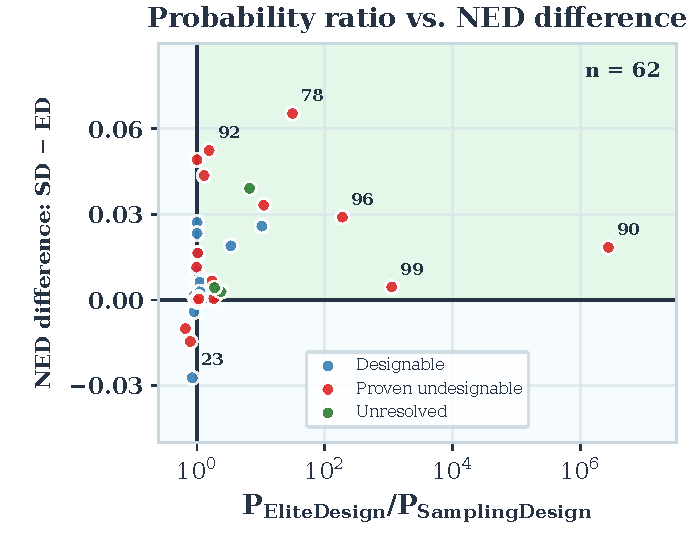
\includegraphics[width=\linewidth]{figures/results/eterna_quadrant_zoom.pdf}
\caption{EliteDesign ($N=500$) versus SamplingDesign on individual Eterna100 puzzles. The $x$-axis is the ratio of their Boltzmann probabilities, and the $y$-axis is SamplingDesign's NED minus EliteDesign's NED. The top right corner shows that EliteDesign is better than SamplingDesign on both metrics for 62 puzzles.}
\label{fig:eterna-advantage}
\end{minipage}\hfill
\begin{minipage}[t]{0.49\textwidth}
\centering
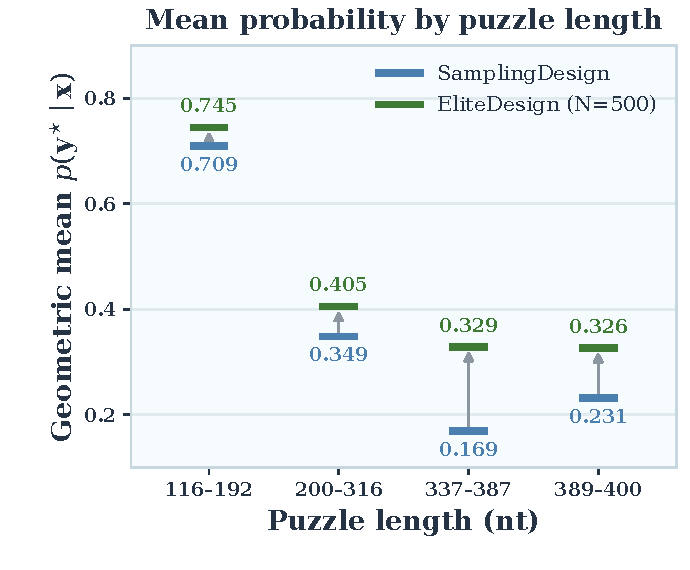
\includegraphics[width=\linewidth]{figures/results/eterna_probability_zoom.pdf}
\caption{Geometric mean Boltzmann probability for the 40 longest Eterna100 puzzles, in four groups of 10 by length. Proven undesignable puzzles are removed from each group, as in SamplingDesign~\citep{tang2026}. The gain from EliteDesign ($N=500$) is largest on long puzzles.}
\label{fig:eterna-length}
\end{minipage}
\end{figure*}

\begin{figure}[H]
\centering
\fbox{\begin{minipage}[c][3.4in][c]{0.94\textwidth}
\centering\textbf{\Large Puzzle 73}
\end{minipage}}\par\smallskip
\textbf{(a)}\par\vspace{0.2in}
\fbox{\begin{minipage}[c][3.4in][c]{0.94\textwidth}
\centering\textbf{\Large Puzzle 76}
\end{minipage}}\par\smallskip
\textbf{(b)}\par\vspace{0.2in}
\caption{}
\label{fig:eterna-structures}
\end{figure}

\clearpage

\subsection{16S rRNA}
\label{sec:results-16s}
\begin{table}[t]
\centering
\renewcommand{\arraystretch}{1.1}
\setlength{\tabcolsep}{3pt}
\begin{tabular}{@{}lccccc@{}}
\toprule
& & \multicolumn{2}{c}{$p(\vecystar\mid\vecx)$ $\uparrow$} & & Time per \\
\cmidrule(lr){3-4}
\textbf{Method} & $N$ & Mean & Geo. & NED $\downarrow$ & \shortstack{target\\(min) $\downarrow$} \\
\midrule
EliteDesign & 100 & 0.510 & 0.480 & 0.0013 & \textbf{39.4} \\
EliteDesign & 500 & \textbf{0.520} & \textbf{0.491} & \textbf{0.0012} & 66.0 \\
\midrule
SAMFEO & --- & 0.185 & 0.129 & --- & 946 \\
\bottomrule
\end{tabular}
\caption{Results on \sixteenS{}, averaged over the ten targets. SAMFEO's results are from our prior work~\citep{zhou2026fastdesign}, which used the same ten targets and did not report NED; the dash marks that omission.}
\label{tab:16s-results}
\end{table}

\begin{figure*}[t]
\centering
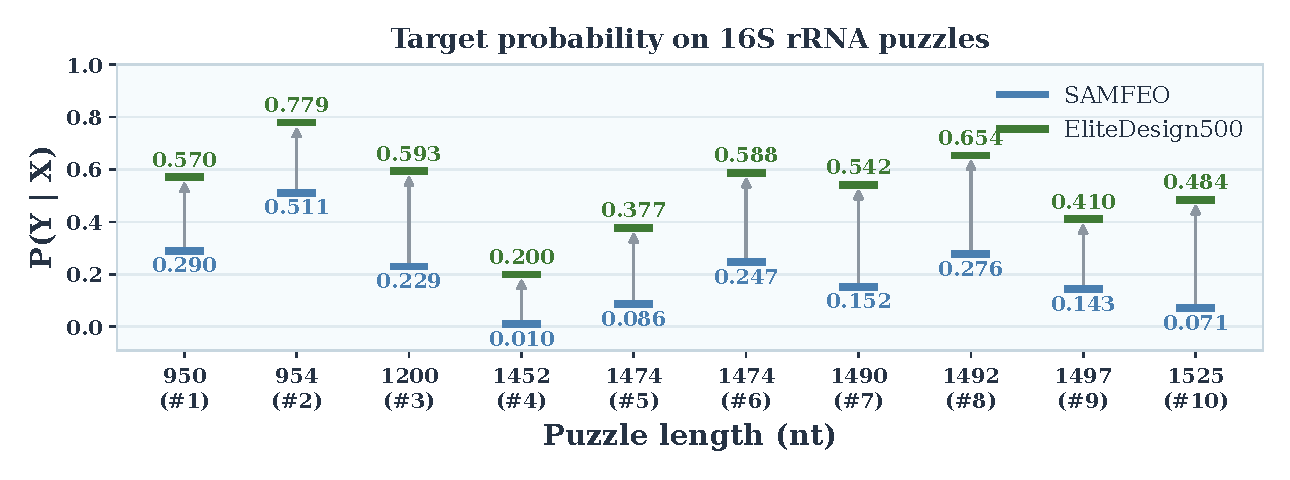
\includegraphics[width=0.88\textwidth]{figures/results/16s_intervals_compact.pdf}
\caption{Boltzmann probability on ten 16S rRNA targets. EliteDesign ($N=500$) is higher than SAMFEO on every target.}
\label{fig:16s-intervals}
\vspace{4pt}
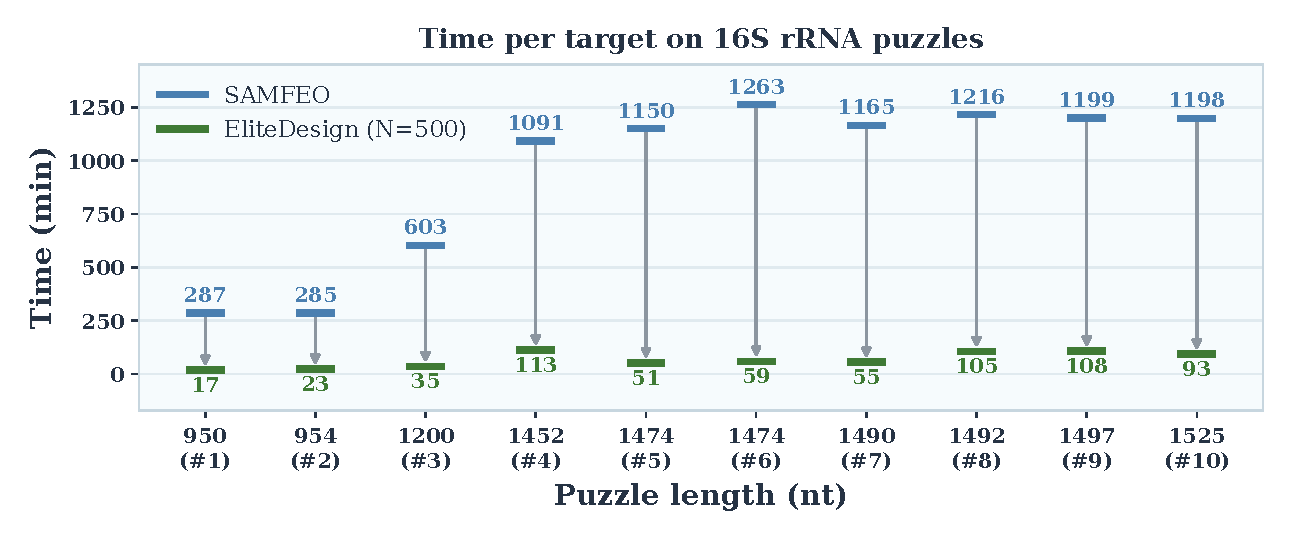
\includegraphics[width=0.88\textwidth]{figures/results/16s_time_vs_size.pdf}
\caption{Time per target in minutes on the same 16S rRNA targets. EliteDesign ($N=500$) is faster than SAMFEO on every target. EliteDesign and SAMFEO were both run on 96-core CPUs, and SAMFEO's times are from \citet{zhou2026fastdesign}.}
\label{fig:16s-time}
\end{figure*}


\twocolumn
